\documentclass{article}

\usepackage{tikz}

\begin{document}
    \title{TikZ pictures (class article)}
    \maketitle

    \providecommand{\psize}[1]{
        \pgfmathparse{#1}
        \pgfmathresult pt
    }
    
    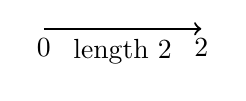
\begin{tikzpicture}
        \draw[thick,->]
        (0,0) node[below] {$0$} 
        --  node[below] {length 2}
        (2,0) node[below] {$2$};
    \end{tikzpicture}
    , a tikzpicture without anything else.

    
    
    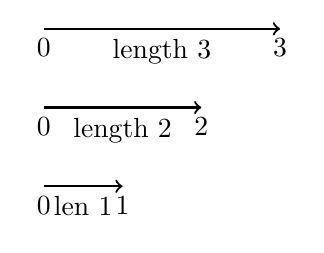
\begin{tikzpicture}
        \draw[yshift=0cm, thick,->] (0,0) node[below] {$0$}  --  node[below] {len    1} (1,0) node[below] {$1$};
        \draw[yshift=1cm, thick,->] (0,0) node[below] {$0$}  --  node[below] {length 2} (2,0) node[below] {$2$};
        \draw[yshift=2cm, thick,->] (0,0) node[below] {$0$}  --  node[below] {length 3} (3,0) node[below] {$3$};
    \end{tikzpicture}
    , a tikzpicture with several lengths.

    
    
    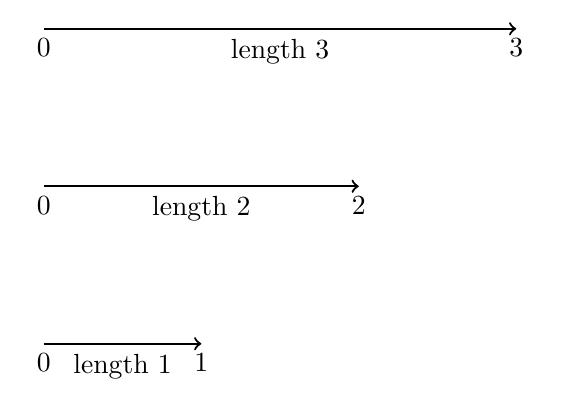
\begin{tikzpicture}[scale=2]
        \draw[yshift=0cm, thick,->] (0,0) node[below] {$0$}  --  node[below] {length 1} (1,0) node[below] {$1$};
        \draw[yshift=1cm, thick,->] (0,0) node[below] {$0$}  --  node[below] {length 2} (2,0) node[below] {$2$};
        \draw[yshift=2cm, thick,->] (0,0) node[below] {$0$}  --  node[below] {length 3} (3,0) node[below] {$3$};
    \end{tikzpicture}
    , a tikzpicture with scale=2.

    
    
    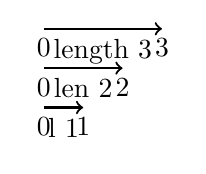
\begin{tikzpicture}[scale=0.5]
        \draw[yshift=0cm, thick,->] (0,0) node[below] {$0$}  --  node[below] {l      1} (1,0) node[below] {$1$};
        \draw[yshift=1cm, thick,->] (0,0) node[below] {$0$}  --  node[below] {len    2} (2,0) node[below] {$2$};
        \draw[yshift=2cm, thick,->] (0,0) node[below] {$0$}  --  node[below] {length 3} (3,0) node[below] {$3$};
    \end{tikzpicture}
    , a tikzpicture with scale=0.5.


    \end{document}